\documentclass{article}

\usepackage[utf8]{inputenc}
\usepackage[T1]{fontenc}
\usepackage{amsmath,amssymb}
\usepackage{textcomp}
\usepackage{float}
\usepackage{listings}
\usepackage{hyperref}
\usepackage{graphicx}
\usepackage[table]{xcolor}
\usepackage{tikz}
\usepackage{pgf-umlcd}
\usetikzlibrary{positioning, fit, calc, shapes, arrows, er}

\definecolor{codegreen}{rgb}{0,0.6,0}
\definecolor{codepurple}{rgb}{0.58,0,0.82}
\definecolor{codegray}{rgb}{0.5,0.5,0.5}

\lstdefinestyle{wstyle}{
    keywordstyle=\color{codepurple},
    stringstyle=\color{codegreen},
    commentstyle=\color{codegray},
}

\lstset{style=wstyle}

\begin{document}

\title{Assingment 1 - Internal DSL}
\author{Marc Bertelsen\\
\textbf{berte20@student.sdu.dk}}

\maketitle

\pagebreak

\section{Desing}

Designing the API for representing state machines, firstly requires abstracting the commonalities present for all state machines, this can be accomplished by creating a metamodel.

\subsection{Metamodel}

Noting what parts, a state machine is made of: the overall state machine itself, the individual states, and the transitions between the states. The state machine has a current state, as well as the possible other states that it can transition to. States have transitions that can happen based on external factors like input and conditional logic. Transition can result in four different outcomes:

\begin{enumerate}
    \item the state machine goes to a new state.
    \item some parameter is updated.
    \item the state machine goes to a new state and parameter update.
    \item the state machine comes to an end.
\end{enumerate}

\begin{figure}[H]
    \centering
    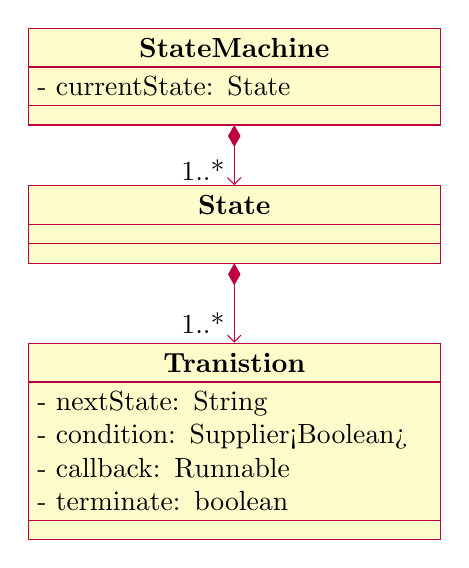
\begin{tikzpicture}
        \begin{class}{StateMachine}{0,0}{
            \attribute{- currentState: State}
        }
        \end{class}
        \begin{class}{State}{0,-2}{
        }
        \end{class}
        \begin{class}{Tranistion}{0,-4}{
            \attribute{- nextState: String}
            \attribute{- condition: Supplier<Boolean>}
            \attribute{- callback: Runnable}
            \attribute{- terminate: boolean}
        }
        \end{class}
        \composition{StateMachine}{}{1..*}{State}
        \composition{State}{}{1..*}{Tranistion}
    \end{tikzpicture}
    \caption{State Machine Metamodel}
\end{figure}

\subsection{Syntax}

The intent is it create a syntax that will read like:\\
''\textbf{Given} the model is in SOME\_STATE, \textbf{when} we give it SOME\_INPUT \textbf{and} SOME\_CONDITION is met/true, \textbf{then} trasition to SOME\_OTHER\_STATE  and/or EXECUTE\_CODE.''\\

\noindent Ideally the example above will translate into code looking like the example seen on fig.~\ref{lst:syntax}.
\begin{lstlisting}[language=java, caption={Example of Intented API Usage}, captionpos=b, label={lst:syntax}]
    statemachine
        .given("SOME_STATE")
            .when("SOME_INPUT")
            .and(() -> true) //SOME_CONDITOIN
            .then("SOME_OTHER_STATE")
            .then(() -> {}) //EXCUTE_CODE
\end{lstlisting}

\textbf{given} - Specify the state the model should be in.
\begin{lstlisting}[language=java]
    T gien(String state);
\end{lstlisting}

\textbf{when} - Specify the input that will cause a transition.
\begin{lstlisting}[language=java]
    T when(String input);
\end{lstlisting}

\textbf{and} - Add an additional constraint that must be met to cause the transition.
\begin{lstlisting}[language=java]
    T and(Supplier<Boolean> condition);
\end{lstlisting}

\textbf{then} - Specify the next state for the transition.
\begin{lstlisting}[language=java]
    T then(String nextState);
\end{lstlisting}

\textbf{then} - Specify some code that will be run with the transition.
\begin{lstlisting}[language=java]
    T then(Runnable callback);
\end{lstlisting}

\textbf{end} - Specify that a transition will lead to an end state.
\begin{lstlisting}[language=java]
    T end();
\end{lstlisting}

\textbf{start} - Specify the initial state.
\begin{lstlisting}[language=java]
    T start(String initialState);
\end{lstlisting}

\subsubsection{Interfaces}

The syntax design results in the \textbf{IStateMachine} interface. Making the interface generic allows for the implementation to specify the return type as itself, which in turn will allow for chaining the method calls.

\begin{lstlisting}[language=java, caption={State Machine Interface}, captionpos=b]
    public interface IStateMachine<T> {
        T given(String state);
        T when(String input);
        T and(Supplier<Boolean> condition);
        T then(String nextState);
        T then(Runnable callback);
        T end();
        T start(String initialState);
    }
\end{lstlisting}

\section{Implmentation}

\textbf{Repo:} \url{https://github.com/Wafl97/MDSD/tree/main/A1/internal_dsl}



\subsection{State Machines}

This subsection features the code representation of the three state machines: CD Player, Microwave Oven, and Cooking Hood. All the code listings featured are simplified from the actual implementations, as to only show the usage of the API.

\subsubsection{CD Player}

\begin{figure}[H]
    \centering
    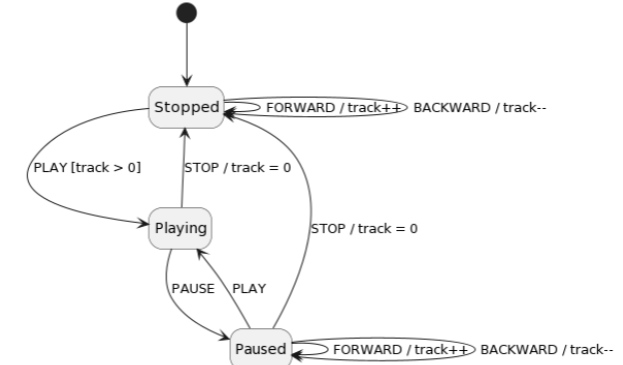
\includegraphics[scale=.75]{./figures/player.PNG}
    \caption{CD Player State Machine Diagram}
\end{figure}

\begin{lstlisting}[language=java, caption={CD Player Implmentation}, captionpos=b]
    new StateMachine("CD PLAYER")

        .given("STOPPED")
            .when("PLAY")
            .and(() -> !trackQueue.isEmpty())
            .then("PLAYING")

            .when("FORWARD")
            .then(() -> trackIndex++)

            .when("BACKWARD")
            .then(() -> trackIndex--)

        .given("PLAYING")
            .when("STOP")
            .then("STOPPED")
            .then(() -> trackIndex = 0)

            .when("PAUSE")
            .then("PAUSED")

        .given("PAUSED")
            .when("PLAY")
            .then("PLAYING")

            .when("STOP")
            .then("STOPPED")
            .then(() -> trackIndex = 0)

            .when("FORWARD")
            .then(() -> trackIndex++)

            .when("BACKWARD")
            .then(() -> trackIndex--)
            
        .start("STOPPED");
\end{lstlisting}

\subsubsection{Micowave Oven}

\begin{figure}[H]
    \centering
    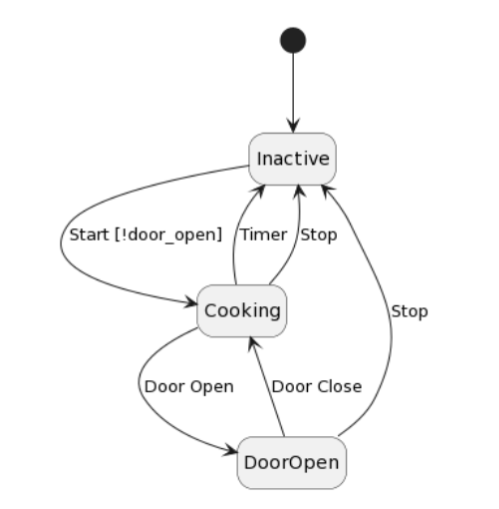
\includegraphics[scale=.75]{./figures/oven.PNG}
    \caption{Microwave Oven State Machine Diagram}
\end{figure}

\begin{lstlisting}[language=java, caption={Microwave Oven Implemntation}, captionpos=b]
    new StateMachine("MICROWAVE OVEN")

        .given("INACTIVE")
            .when("START")
            .and(() -> !doorOpen)
            .then("COOKING")

        .given("COOKING")
            .when("TIMER")
            .then("INACTIVE")

            .when("STOP")
            .then("INACTIVE")

            .when("OPEN_DOOR")
            .then("DOOR_OPEN")
            .then(() -> doorOpen = true)

        .given("DOOR_OPEN")
            .when("CLOSE_DOOR")
            .then(() -> doorOpen = true)
            .then("COOKING")

            .when("STOP")
            .then("INACTIVE")
            
        .start("INACTIVE");
\end{lstlisting}

\subsubsection{Cooking Hood}

\begin{figure}[H]
    \centering
    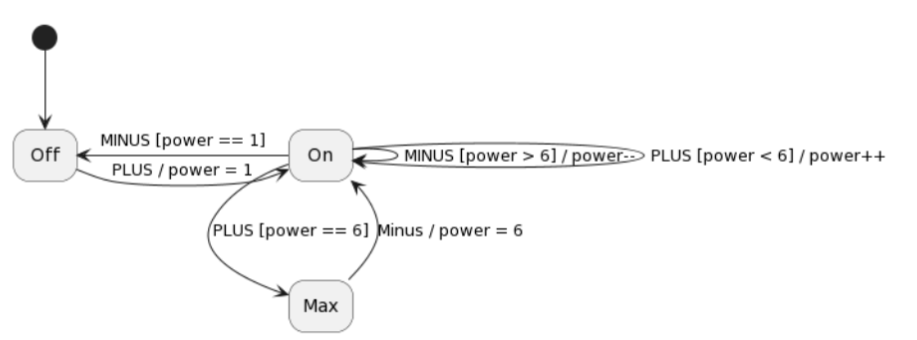
\includegraphics[scale=.60]{./figures/hood.PNG}
    \caption{Cooking Hood State Machine Diagram}
\end{figure}

\begin{lstlisting}[language=java, caption={Cooking Hood Implmentation}, captionpos=b]
    new StateMachine("COOKING HOOD")

        .given("OFF")
            .when("PLUS")
            .then("ON")
            .then(() -> power = 1)

        .given("ON")
            .when("MINUS")
            .and(() -> power == 1)
            .then("OFF")

            .when("PLUS")
            .and(() -> power == 6)
            .then("MAX")

            .when("PLUS")
            .and(() -> power < 6)
            .then(() -> power++)

            .when("MINUS")
            .and(() -> power == 1)
            .then("OFF")

            .when("MINUS")
            .and(() -> power > 0)
            .then(() -> power--)

        .given("MAX")
            .when("MINUS")
            .then("ON")
            .then(() -> power = 6)
        
        .start("OFF");
\end{lstlisting}

\section{Test}

For the purpose of testing, three additional methods are added to the state machine implementation: i(input), o(output), and printMode. These allow for configuring the input and output for the state machine, as well as how much info it outputs. Default for input and output is \textbf{System.in} and \textbf{System.out}, respectively, with printMode defaulting to \textbf{NORMAL}.

\subsection{Simulating Input and Output}

A queue is used to simulate the input for the state machines in the various tests. This way it will be possible to structure and ensure the order of each command to the state machine. For the output, a list is used to collect everything from the state machine. This output list is then compared with a predefined list with the expected outputs. Additionally, the print mode is set to \textbf{TESTING}, so only the state and errors are given as output.

\begin{lstlisting}[language=java, caption={Input and Output Test Setup}, captionpos=b,]
    final Queue<String> simulatedInputs = new LinkedList<>()
    {{
        add("A");
        // structure of inputs
        // ...
    }};
    final Queue<String> simulatedOutputs = new LinkedList<>();
    final Queue<String> expectedOutputs = new LinkedList<>()
    {{
        add("STATE_A");
        // structure of expeced output
        // ...
    }};

    new StateMachine("GENERIC MODEL")
            .printMode(PrintMode.TESTING)
            .i(simulatedInputs::poll)
            .o(simulatedOutputs::add)
            // state machine logic
            // ...

    // state machine has terminated
    assertEquals(
        expectedOutputs.size(), simulatedOutputs.size());

    assertArrayEquals(
        expectedOutputs.toArray(), simulatedOutputs.toArray());       
\end{lstlisting}

Different tests have been written to test the flow from state to state, as well as testing for bad/wrong input. On fig.~\ref{fig:test_cov} the total coverage of the tests can be seen, with the only remaining code being print statements never reached while the printMode is \textbf{TESTING}.

\begin{figure}[H]
    \centering
    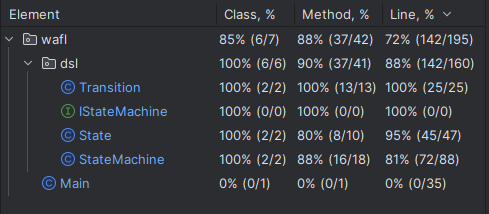
\includegraphics{figures/tests.PNG}
    \caption{Test Coverage}
    \label{fig:test_cov}
\end{figure}

\section{Conclusion}

The resulting API is able to capture the logic from all three state machine diagrams, in addition to the main program having a state machine for selecting each of the implementations to run. So, the API is usable for its intended purpose.\\
Creating an API based on the commonalities of the different state machines, made implementing each trivial, with the added benefit of easily being able to add and change the logic without huge refactors.

\end{document}